% Created by tikzDevice version 0.12.6 on 2025-02-14 03:12:03
% !TEX encoding = UTF-8 Unicode
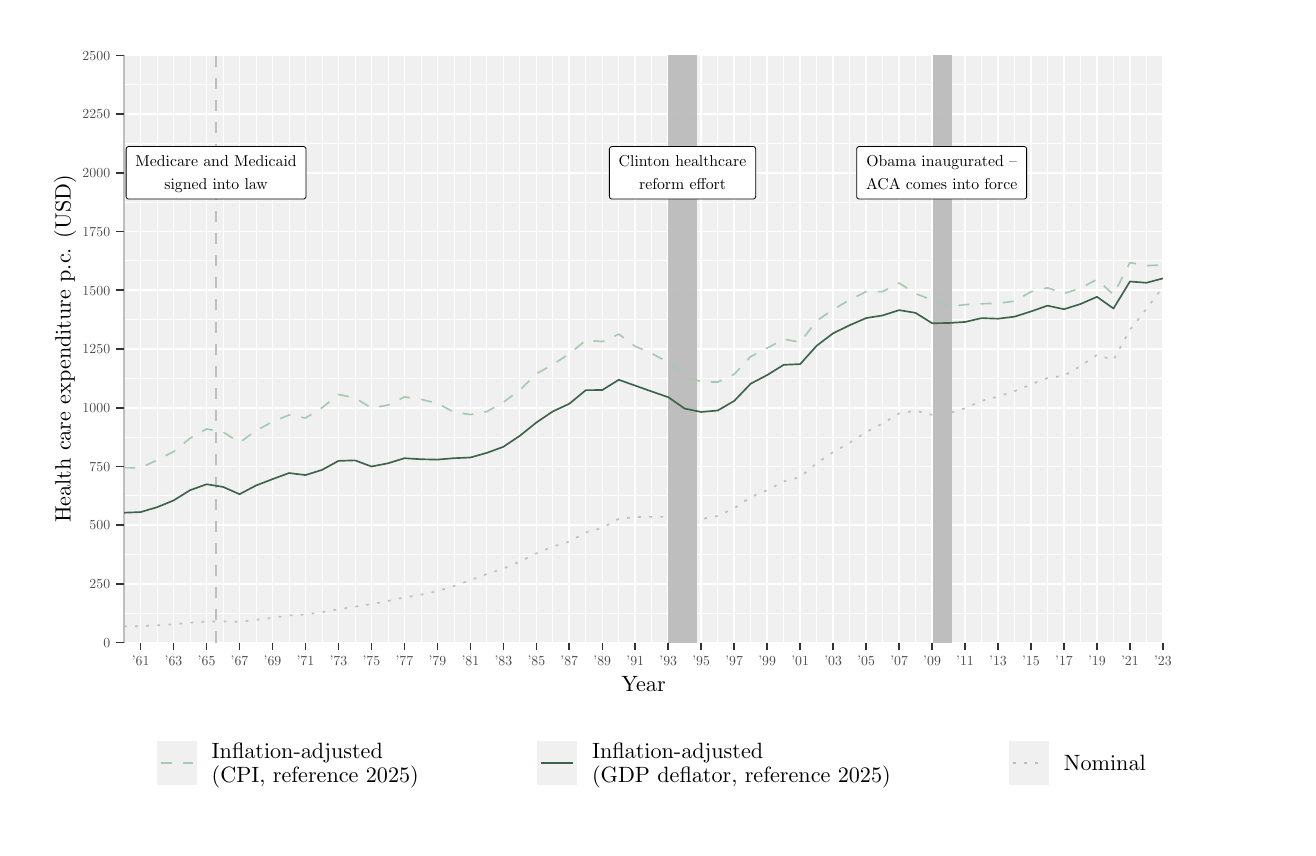
\begin{tikzpicture}[x=1pt,y=1pt]
\definecolor{fillColor}{RGB}{255,255,255}
\path[use as bounding box,fill=fillColor,fill opacity=0.00] (0,0) rectangle (455.30,289.08);
\begin{scope}
\path[clip] (  0.00,  0.00) rectangle (455.30,289.08);
\definecolor{drawColor}{RGB}{255,255,255}
\definecolor{fillColor}{RGB}{255,255,255}

\path[draw=drawColor,line width= 0.6pt,line join=round,line cap=round,fill=fillColor] ( -0.00,  0.00) rectangle (455.30,289.08);
\end{scope}
\begin{scope}
\path[clip] (  0.00,  0.00) rectangle (455.30,289.08);
\definecolor{fillColor}{gray}{0.94}

\path[fill=fillColor] ( 34.76, 66.89) rectangle (410.30,279.08);
\definecolor{drawColor}{RGB}{255,255,255}

\path[draw=drawColor,line width= 0.3pt,line join=round] ( 34.76, 77.50) --
	(410.30, 77.50);

\path[draw=drawColor,line width= 0.3pt,line join=round] ( 34.76, 98.71) --
	(410.30, 98.71);

\path[draw=drawColor,line width= 0.3pt,line join=round] ( 34.76,119.93) --
	(410.30,119.93);

\path[draw=drawColor,line width= 0.3pt,line join=round] ( 34.76,141.15) --
	(410.30,141.15);

\path[draw=drawColor,line width= 0.3pt,line join=round] ( 34.76,162.37) --
	(410.30,162.37);

\path[draw=drawColor,line width= 0.3pt,line join=round] ( 34.76,183.59) --
	(410.30,183.59);

\path[draw=drawColor,line width= 0.3pt,line join=round] ( 34.76,204.81) --
	(410.30,204.81);

\path[draw=drawColor,line width= 0.3pt,line join=round] ( 34.76,226.03) --
	(410.30,226.03);

\path[draw=drawColor,line width= 0.3pt,line join=round] ( 34.76,247.25) --
	(410.30,247.25);

\path[draw=drawColor,line width= 0.3pt,line join=round] ( 34.76,268.47) --
	(410.30,268.47);

\path[draw=drawColor,line width= 0.3pt,line join=round] ( 34.85, 66.89) --
	( 34.85,279.08);

\path[draw=drawColor,line width= 0.3pt,line join=round] ( 46.77, 66.89) --
	( 46.77,279.08);

\path[draw=drawColor,line width= 0.3pt,line join=round] ( 58.69, 66.89) --
	( 58.69,279.08);

\path[draw=drawColor,line width= 0.3pt,line join=round] ( 70.60, 66.89) --
	( 70.60,279.08);

\path[draw=drawColor,line width= 0.3pt,line join=round] ( 82.52, 66.89) --
	( 82.52,279.08);

\path[draw=drawColor,line width= 0.3pt,line join=round] ( 94.43, 66.89) --
	( 94.43,279.08);

\path[draw=drawColor,line width= 0.3pt,line join=round] (106.35, 66.89) --
	(106.35,279.08);

\path[draw=drawColor,line width= 0.3pt,line join=round] (118.27, 66.89) --
	(118.27,279.08);

\path[draw=drawColor,line width= 0.3pt,line join=round] (130.18, 66.89) --
	(130.18,279.08);

\path[draw=drawColor,line width= 0.3pt,line join=round] (142.10, 66.89) --
	(142.10,279.08);

\path[draw=drawColor,line width= 0.3pt,line join=round] (154.02, 66.89) --
	(154.02,279.08);

\path[draw=drawColor,line width= 0.3pt,line join=round] (165.93, 66.89) --
	(165.93,279.08);

\path[draw=drawColor,line width= 0.3pt,line join=round] (177.85, 66.89) --
	(177.85,279.08);

\path[draw=drawColor,line width= 0.3pt,line join=round] (189.77, 66.89) --
	(189.77,279.08);

\path[draw=drawColor,line width= 0.3pt,line join=round] (201.68, 66.89) --
	(201.68,279.08);

\path[draw=drawColor,line width= 0.3pt,line join=round] (213.60, 66.89) --
	(213.60,279.08);

\path[draw=drawColor,line width= 0.3pt,line join=round] (225.52, 66.89) --
	(225.52,279.08);

\path[draw=drawColor,line width= 0.3pt,line join=round] (237.43, 66.89) --
	(237.43,279.08);

\path[draw=drawColor,line width= 0.3pt,line join=round] (249.35, 66.89) --
	(249.35,279.08);

\path[draw=drawColor,line width= 0.3pt,line join=round] (261.27, 66.89) --
	(261.27,279.08);

\path[draw=drawColor,line width= 0.3pt,line join=round] (273.18, 66.89) --
	(273.18,279.08);

\path[draw=drawColor,line width= 0.3pt,line join=round] (285.10, 66.89) --
	(285.10,279.08);

\path[draw=drawColor,line width= 0.3pt,line join=round] (297.02, 66.89) --
	(297.02,279.08);

\path[draw=drawColor,line width= 0.3pt,line join=round] (308.93, 66.89) --
	(308.93,279.08);

\path[draw=drawColor,line width= 0.3pt,line join=round] (320.85, 66.89) --
	(320.85,279.08);

\path[draw=drawColor,line width= 0.3pt,line join=round] (332.77, 66.89) --
	(332.77,279.08);

\path[draw=drawColor,line width= 0.3pt,line join=round] (344.68, 66.89) --
	(344.68,279.08);

\path[draw=drawColor,line width= 0.3pt,line join=round] (356.60, 66.89) --
	(356.60,279.08);

\path[draw=drawColor,line width= 0.3pt,line join=round] (368.52, 66.89) --
	(368.52,279.08);

\path[draw=drawColor,line width= 0.3pt,line join=round] (380.43, 66.89) --
	(380.43,279.08);

\path[draw=drawColor,line width= 0.3pt,line join=round] (392.35, 66.89) --
	(392.35,279.08);

\path[draw=drawColor,line width= 0.3pt,line join=round] (404.27, 66.89) --
	(404.27,279.08);

\path[draw=drawColor,line width= 0.6pt,line join=round] ( 34.76, 66.89) --
	(410.30, 66.89);

\path[draw=drawColor,line width= 0.6pt,line join=round] ( 34.76, 88.10) --
	(410.30, 88.10);

\path[draw=drawColor,line width= 0.6pt,line join=round] ( 34.76,109.32) --
	(410.30,109.32);

\path[draw=drawColor,line width= 0.6pt,line join=round] ( 34.76,130.54) --
	(410.30,130.54);

\path[draw=drawColor,line width= 0.6pt,line join=round] ( 34.76,151.76) --
	(410.30,151.76);

\path[draw=drawColor,line width= 0.6pt,line join=round] ( 34.76,172.98) --
	(410.30,172.98);

\path[draw=drawColor,line width= 0.6pt,line join=round] ( 34.76,194.20) --
	(410.30,194.20);

\path[draw=drawColor,line width= 0.6pt,line join=round] ( 34.76,215.42) --
	(410.30,215.42);

\path[draw=drawColor,line width= 0.6pt,line join=round] ( 34.76,236.64) --
	(410.30,236.64);

\path[draw=drawColor,line width= 0.6pt,line join=round] ( 34.76,257.86) --
	(410.30,257.86);

\path[draw=drawColor,line width= 0.6pt,line join=round] ( 34.76,279.08) --
	(410.30,279.08);

\path[draw=drawColor,line width= 0.6pt,line join=round] ( 40.81, 66.89) --
	( 40.81,279.08);

\path[draw=drawColor,line width= 0.6pt,line join=round] ( 52.72, 66.89) --
	( 52.72,279.08);

\path[draw=drawColor,line width= 0.6pt,line join=round] ( 64.65, 66.89) --
	( 64.65,279.08);

\path[draw=drawColor,line width= 0.6pt,line join=round] ( 76.56, 66.89) --
	( 76.56,279.08);

\path[draw=drawColor,line width= 0.6pt,line join=round] ( 88.48, 66.89) --
	( 88.48,279.08);

\path[draw=drawColor,line width= 0.6pt,line join=round] (100.39, 66.89) --
	(100.39,279.08);

\path[draw=drawColor,line width= 0.6pt,line join=round] (112.31, 66.89) --
	(112.31,279.08);

\path[draw=drawColor,line width= 0.6pt,line join=round] (124.22, 66.89) --
	(124.22,279.08);

\path[draw=drawColor,line width= 0.6pt,line join=round] (136.15, 66.89) --
	(136.15,279.08);

\path[draw=drawColor,line width= 0.6pt,line join=round] (148.06, 66.89) --
	(148.06,279.08);

\path[draw=drawColor,line width= 0.6pt,line join=round] (159.98, 66.89) --
	(159.98,279.08);

\path[draw=drawColor,line width= 0.6pt,line join=round] (171.89, 66.89) --
	(171.89,279.08);

\path[draw=drawColor,line width= 0.6pt,line join=round] (183.81, 66.89) --
	(183.81,279.08);

\path[draw=drawColor,line width= 0.6pt,line join=round] (195.72, 66.89) --
	(195.72,279.08);

\path[draw=drawColor,line width= 0.6pt,line join=round] (207.65, 66.89) --
	(207.65,279.08);

\path[draw=drawColor,line width= 0.6pt,line join=round] (219.55, 66.89) --
	(219.55,279.08);

\path[draw=drawColor,line width= 0.6pt,line join=round] (231.48, 66.89) --
	(231.48,279.08);

\path[draw=drawColor,line width= 0.6pt,line join=round] (243.39, 66.89) --
	(243.39,279.08);

\path[draw=drawColor,line width= 0.6pt,line join=round] (255.31, 66.89) --
	(255.31,279.08);

\path[draw=drawColor,line width= 0.6pt,line join=round] (267.22, 66.89) --
	(267.22,279.08);

\path[draw=drawColor,line width= 0.6pt,line join=round] (279.15, 66.89) --
	(279.15,279.08);

\path[draw=drawColor,line width= 0.6pt,line join=round] (291.05, 66.89) --
	(291.05,279.08);

\path[draw=drawColor,line width= 0.6pt,line join=round] (302.98, 66.89) --
	(302.98,279.08);

\path[draw=drawColor,line width= 0.6pt,line join=round] (314.89, 66.89) --
	(314.89,279.08);

\path[draw=drawColor,line width= 0.6pt,line join=round] (326.81, 66.89) --
	(326.81,279.08);

\path[draw=drawColor,line width= 0.6pt,line join=round] (338.72, 66.89) --
	(338.72,279.08);

\path[draw=drawColor,line width= 0.6pt,line join=round] (350.64, 66.89) --
	(350.64,279.08);

\path[draw=drawColor,line width= 0.6pt,line join=round] (362.55, 66.89) --
	(362.55,279.08);

\path[draw=drawColor,line width= 0.6pt,line join=round] (374.48, 66.89) --
	(374.48,279.08);

\path[draw=drawColor,line width= 0.6pt,line join=round] (386.39, 66.89) --
	(386.39,279.08);

\path[draw=drawColor,line width= 0.6pt,line join=round] (398.31, 66.89) --
	(398.31,279.08);

\path[draw=drawColor,line width= 0.6pt,line join=round] (410.22, 66.89) --
	(410.22,279.08);
\definecolor{drawColor}{RGB}{190,190,190}

\path[draw=drawColor,line width= 0.6pt,line join=round] ( 34.84, 66.89) -- ( 34.84,279.08);
\definecolor{fillColor}{RGB}{190,190,190}

\path[fill=fillColor,fill opacity=0.01] (231.48, 66.89) rectangle (241.81,279.08);

\path[fill=fillColor,fill opacity=0.01] (231.48, 66.89) rectangle (241.81,279.08);

\path[fill=fillColor,fill opacity=0.01] (231.48, 66.89) rectangle (241.81,279.08);

\path[fill=fillColor,fill opacity=0.01] (231.48, 66.89) rectangle (241.81,279.08);

\path[fill=fillColor,fill opacity=0.01] (231.48, 66.89) rectangle (241.81,279.08);

\path[fill=fillColor,fill opacity=0.01] (231.48, 66.89) rectangle (241.81,279.08);

\path[fill=fillColor,fill opacity=0.01] (231.48, 66.89) rectangle (241.81,279.08);

\path[fill=fillColor,fill opacity=0.01] (231.48, 66.89) rectangle (241.81,279.08);

\path[fill=fillColor,fill opacity=0.01] (231.48, 66.89) rectangle (241.81,279.08);

\path[fill=fillColor,fill opacity=0.01] (231.48, 66.89) rectangle (241.81,279.08);

\path[fill=fillColor,fill opacity=0.01] (231.48, 66.89) rectangle (241.81,279.08);

\path[fill=fillColor,fill opacity=0.01] (231.48, 66.89) rectangle (241.81,279.08);

\path[fill=fillColor,fill opacity=0.01] (231.48, 66.89) rectangle (241.81,279.08);

\path[fill=fillColor,fill opacity=0.01] (231.48, 66.89) rectangle (241.81,279.08);

\path[fill=fillColor,fill opacity=0.01] (231.48, 66.89) rectangle (241.81,279.08);

\path[fill=fillColor,fill opacity=0.01] (231.48, 66.89) rectangle (241.81,279.08);

\path[fill=fillColor,fill opacity=0.01] (231.48, 66.89) rectangle (241.81,279.08);

\path[fill=fillColor,fill opacity=0.01] (231.48, 66.89) rectangle (241.81,279.08);

\path[fill=fillColor,fill opacity=0.01] (231.48, 66.89) rectangle (241.81,279.08);

\path[fill=fillColor,fill opacity=0.01] (231.48, 66.89) rectangle (241.81,279.08);

\path[fill=fillColor,fill opacity=0.01] (231.48, 66.89) rectangle (241.81,279.08);

\path[fill=fillColor,fill opacity=0.01] (231.48, 66.89) rectangle (241.81,279.08);

\path[fill=fillColor,fill opacity=0.01] (231.48, 66.89) rectangle (241.81,279.08);

\path[fill=fillColor,fill opacity=0.01] (231.48, 66.89) rectangle (241.81,279.08);

\path[fill=fillColor,fill opacity=0.01] (231.48, 66.89) rectangle (241.81,279.08);

\path[fill=fillColor,fill opacity=0.01] (231.48, 66.89) rectangle (241.81,279.08);

\path[fill=fillColor,fill opacity=0.01] (231.48, 66.89) rectangle (241.81,279.08);

\path[fill=fillColor,fill opacity=0.01] (231.48, 66.89) rectangle (241.81,279.08);

\path[fill=fillColor,fill opacity=0.01] (231.48, 66.89) rectangle (241.81,279.08);

\path[fill=fillColor,fill opacity=0.01] (231.48, 66.89) rectangle (241.81,279.08);

\path[fill=fillColor,fill opacity=0.01] (231.48, 66.89) rectangle (241.81,279.08);

\path[fill=fillColor,fill opacity=0.01] (231.48, 66.89) rectangle (241.81,279.08);

\path[fill=fillColor,fill opacity=0.01] (231.48, 66.89) rectangle (241.81,279.08);

\path[fill=fillColor,fill opacity=0.01] (231.48, 66.89) rectangle (241.81,279.08);

\path[fill=fillColor,fill opacity=0.01] (231.48, 66.89) rectangle (241.81,279.08);

\path[fill=fillColor,fill opacity=0.01] (231.48, 66.89) rectangle (241.81,279.08);

\path[fill=fillColor,fill opacity=0.01] (231.48, 66.89) rectangle (241.81,279.08);

\path[fill=fillColor,fill opacity=0.01] (231.48, 66.89) rectangle (241.81,279.08);

\path[fill=fillColor,fill opacity=0.01] (231.48, 66.89) rectangle (241.81,279.08);

\path[fill=fillColor,fill opacity=0.01] (231.48, 66.89) rectangle (241.81,279.08);

\path[fill=fillColor,fill opacity=0.01] (231.48, 66.89) rectangle (241.81,279.08);

\path[fill=fillColor,fill opacity=0.01] (231.48, 66.89) rectangle (241.81,279.08);

\path[fill=fillColor,fill opacity=0.01] (231.48, 66.89) rectangle (241.81,279.08);

\path[fill=fillColor,fill opacity=0.01] (231.48, 66.89) rectangle (241.81,279.08);

\path[fill=fillColor,fill opacity=0.01] (231.48, 66.89) rectangle (241.81,279.08);

\path[fill=fillColor,fill opacity=0.01] (231.48, 66.89) rectangle (241.81,279.08);

\path[fill=fillColor,fill opacity=0.01] (231.48, 66.89) rectangle (241.81,279.08);

\path[fill=fillColor,fill opacity=0.01] (231.48, 66.89) rectangle (241.81,279.08);

\path[fill=fillColor,fill opacity=0.01] (231.48, 66.89) rectangle (241.81,279.08);

\path[fill=fillColor,fill opacity=0.01] (231.48, 66.89) rectangle (241.81,279.08);

\path[fill=fillColor,fill opacity=0.01] (231.48, 66.89) rectangle (241.81,279.08);

\path[fill=fillColor,fill opacity=0.01] (231.48, 66.89) rectangle (241.81,279.08);

\path[fill=fillColor,fill opacity=0.01] (231.48, 66.89) rectangle (241.81,279.08);

\path[fill=fillColor,fill opacity=0.01] (231.48, 66.89) rectangle (241.81,279.08);

\path[fill=fillColor,fill opacity=0.01] (231.48, 66.89) rectangle (241.81,279.08);

\path[fill=fillColor,fill opacity=0.01] (231.48, 66.89) rectangle (241.81,279.08);

\path[fill=fillColor,fill opacity=0.01] (231.48, 66.89) rectangle (241.81,279.08);

\path[fill=fillColor,fill opacity=0.01] (231.48, 66.89) rectangle (241.81,279.08);

\path[fill=fillColor,fill opacity=0.01] (231.48, 66.89) rectangle (241.81,279.08);

\path[fill=fillColor,fill opacity=0.01] (231.48, 66.89) rectangle (241.81,279.08);

\path[fill=fillColor,fill opacity=0.01] (231.48, 66.89) rectangle (241.81,279.08);

\path[fill=fillColor,fill opacity=0.01] (231.48, 66.89) rectangle (241.81,279.08);

\path[fill=fillColor,fill opacity=0.01] (231.48, 66.89) rectangle (241.81,279.08);

\path[fill=fillColor,fill opacity=0.01] (231.48, 66.89) rectangle (241.81,279.08);

\path[fill=fillColor,fill opacity=0.01] (327.12, 66.89) rectangle (334.09,279.08);

\path[fill=fillColor,fill opacity=0.01] (327.12, 66.89) rectangle (334.09,279.08);

\path[fill=fillColor,fill opacity=0.01] (327.12, 66.89) rectangle (334.09,279.08);

\path[fill=fillColor,fill opacity=0.01] (327.12, 66.89) rectangle (334.09,279.08);

\path[fill=fillColor,fill opacity=0.01] (327.12, 66.89) rectangle (334.09,279.08);

\path[fill=fillColor,fill opacity=0.01] (327.12, 66.89) rectangle (334.09,279.08);

\path[fill=fillColor,fill opacity=0.01] (327.12, 66.89) rectangle (334.09,279.08);

\path[fill=fillColor,fill opacity=0.01] (327.12, 66.89) rectangle (334.09,279.08);

\path[fill=fillColor,fill opacity=0.01] (327.12, 66.89) rectangle (334.09,279.08);

\path[fill=fillColor,fill opacity=0.01] (327.12, 66.89) rectangle (334.09,279.08);

\path[fill=fillColor,fill opacity=0.01] (327.12, 66.89) rectangle (334.09,279.08);

\path[fill=fillColor,fill opacity=0.01] (327.12, 66.89) rectangle (334.09,279.08);

\path[fill=fillColor,fill opacity=0.01] (327.12, 66.89) rectangle (334.09,279.08);

\path[fill=fillColor,fill opacity=0.01] (327.12, 66.89) rectangle (334.09,279.08);

\path[fill=fillColor,fill opacity=0.01] (327.12, 66.89) rectangle (334.09,279.08);

\path[fill=fillColor,fill opacity=0.01] (327.12, 66.89) rectangle (334.09,279.08);

\path[fill=fillColor,fill opacity=0.01] (327.12, 66.89) rectangle (334.09,279.08);

\path[fill=fillColor,fill opacity=0.01] (327.12, 66.89) rectangle (334.09,279.08);

\path[fill=fillColor,fill opacity=0.01] (327.12, 66.89) rectangle (334.09,279.08);

\path[fill=fillColor,fill opacity=0.01] (327.12, 66.89) rectangle (334.09,279.08);

\path[fill=fillColor,fill opacity=0.01] (327.12, 66.89) rectangle (334.09,279.08);

\path[fill=fillColor,fill opacity=0.01] (327.12, 66.89) rectangle (334.09,279.08);

\path[fill=fillColor,fill opacity=0.01] (327.12, 66.89) rectangle (334.09,279.08);

\path[fill=fillColor,fill opacity=0.01] (327.12, 66.89) rectangle (334.09,279.08);

\path[fill=fillColor,fill opacity=0.01] (327.12, 66.89) rectangle (334.09,279.08);

\path[fill=fillColor,fill opacity=0.01] (327.12, 66.89) rectangle (334.09,279.08);

\path[fill=fillColor,fill opacity=0.01] (327.12, 66.89) rectangle (334.09,279.08);

\path[fill=fillColor,fill opacity=0.01] (327.12, 66.89) rectangle (334.09,279.08);

\path[fill=fillColor,fill opacity=0.01] (327.12, 66.89) rectangle (334.09,279.08);

\path[fill=fillColor,fill opacity=0.01] (327.12, 66.89) rectangle (334.09,279.08);

\path[fill=fillColor,fill opacity=0.01] (327.12, 66.89) rectangle (334.09,279.08);

\path[fill=fillColor,fill opacity=0.01] (327.12, 66.89) rectangle (334.09,279.08);

\path[fill=fillColor,fill opacity=0.01] (327.12, 66.89) rectangle (334.09,279.08);

\path[fill=fillColor,fill opacity=0.01] (327.12, 66.89) rectangle (334.09,279.08);

\path[fill=fillColor,fill opacity=0.01] (327.12, 66.89) rectangle (334.09,279.08);

\path[fill=fillColor,fill opacity=0.01] (327.12, 66.89) rectangle (334.09,279.08);

\path[fill=fillColor,fill opacity=0.01] (327.12, 66.89) rectangle (334.09,279.08);

\path[fill=fillColor,fill opacity=0.01] (327.12, 66.89) rectangle (334.09,279.08);

\path[fill=fillColor,fill opacity=0.01] (327.12, 66.89) rectangle (334.09,279.08);

\path[fill=fillColor,fill opacity=0.01] (327.12, 66.89) rectangle (334.09,279.08);

\path[fill=fillColor,fill opacity=0.01] (327.12, 66.89) rectangle (334.09,279.08);

\path[fill=fillColor,fill opacity=0.01] (327.12, 66.89) rectangle (334.09,279.08);

\path[fill=fillColor,fill opacity=0.01] (327.12, 66.89) rectangle (334.09,279.08);

\path[fill=fillColor,fill opacity=0.01] (327.12, 66.89) rectangle (334.09,279.08);

\path[fill=fillColor,fill opacity=0.01] (327.12, 66.89) rectangle (334.09,279.08);

\path[fill=fillColor,fill opacity=0.01] (327.12, 66.89) rectangle (334.09,279.08);

\path[fill=fillColor,fill opacity=0.01] (327.12, 66.89) rectangle (334.09,279.08);

\path[fill=fillColor,fill opacity=0.01] (327.12, 66.89) rectangle (334.09,279.08);

\path[fill=fillColor,fill opacity=0.01] (327.12, 66.89) rectangle (334.09,279.08);

\path[fill=fillColor,fill opacity=0.01] (327.12, 66.89) rectangle (334.09,279.08);

\path[fill=fillColor,fill opacity=0.01] (327.12, 66.89) rectangle (334.09,279.08);

\path[fill=fillColor,fill opacity=0.01] (327.12, 66.89) rectangle (334.09,279.08);

\path[fill=fillColor,fill opacity=0.01] (327.12, 66.89) rectangle (334.09,279.08);

\path[fill=fillColor,fill opacity=0.01] (327.12, 66.89) rectangle (334.09,279.08);

\path[fill=fillColor,fill opacity=0.01] (327.12, 66.89) rectangle (334.09,279.08);

\path[fill=fillColor,fill opacity=0.01] (327.12, 66.89) rectangle (334.09,279.08);

\path[fill=fillColor,fill opacity=0.01] (327.12, 66.89) rectangle (334.09,279.08);

\path[fill=fillColor,fill opacity=0.01] (327.12, 66.89) rectangle (334.09,279.08);

\path[fill=fillColor,fill opacity=0.01] (327.12, 66.89) rectangle (334.09,279.08);

\path[fill=fillColor,fill opacity=0.01] (327.12, 66.89) rectangle (334.09,279.08);

\path[fill=fillColor,fill opacity=0.01] (327.12, 66.89) rectangle (334.09,279.08);

\path[fill=fillColor,fill opacity=0.01] (327.12, 66.89) rectangle (334.09,279.08);

\path[fill=fillColor,fill opacity=0.01] (327.12, 66.89) rectangle (334.09,279.08);

\path[fill=fillColor,fill opacity=0.01] (327.12, 66.89) rectangle (334.09,279.08);

\path[draw=drawColor,line width= 0.6pt,dash pattern=on 4pt off 4pt ,line join=round] ( 68.07, 66.89) -- ( 68.07,279.08);
\definecolor{drawColor}{RGB}{0,0,0}
\definecolor{fillColor}{RGB}{255,255,255}

\path[draw=drawColor,line width= 0.3pt,line join=round,line cap=round,fill=fillColor] ( 36.59,227.16) --
	( 99.56,227.16) --
	( 99.52,227.16) --
	( 99.68,227.16) --
	( 99.85,227.20) --
	(100.00,227.26) --
	(100.14,227.34) --
	(100.27,227.44) --
	(100.38,227.57) --
	(100.47,227.71) --
	(100.54,227.86) --
	(100.58,228.02) --
	(100.59,228.19) --
	(100.59,228.19) --
	(100.59,245.10) --
	(100.59,245.10) --
	(100.58,245.26) --
	(100.54,245.42) --
	(100.47,245.57) --
	(100.38,245.71) --
	(100.27,245.84) --
	(100.14,245.94) --
	(100.00,246.03) --
	( 99.85,246.08) --
	( 99.68,246.12) --
	( 99.56,246.13) --
	( 36.59,246.13) --
	( 36.71,246.12) --
	( 36.54,246.12) --
	( 36.38,246.10) --
	( 36.22,246.06) --
	( 36.07,245.99) --
	( 35.94,245.89) --
	( 35.82,245.78) --
	( 35.72,245.65) --
	( 35.64,245.50) --
	( 35.59,245.34) --
	( 35.56,245.18) --
	( 35.56,245.10) --
	( 35.56,228.19) --
	( 35.56,228.27) --
	( 35.56,228.10) --
	( 35.59,227.94) --
	( 35.64,227.78) --
	( 35.72,227.64) --
	( 35.82,227.50) --
	( 35.94,227.39) --
	( 36.07,227.29) --
	( 36.22,227.22) --
	( 36.38,227.18) --
	( 36.54,227.16) --
	cycle;
\end{scope}
\begin{scope}
\path[clip] (  0.00,  0.00) rectangle (455.30,289.08);
\definecolor{drawColor}{RGB}{0,0,0}

\node[text=drawColor,anchor=base,inner sep=0pt, outer sep=0pt, scale=  0.57] at ( 68.07,238.78) {Medicare and Medicaid };

\node[text=drawColor,anchor=base,inner sep=0pt, outer sep=0pt, scale=  0.57] at ( 68.07,230.58) { signed into law};
\end{scope}
\begin{scope}
\path[clip] (  0.00,  0.00) rectangle (455.30,289.08);
\definecolor{drawColor}{RGB}{0,0,0}
\definecolor{fillColor}{RGB}{255,255,255}

\path[draw=drawColor,line width= 0.3pt,line join=round,line cap=round,fill=fillColor] (211.23,227.16) --
	(262.04,227.16) --
	(262.00,227.16) --
	(262.16,227.16) --
	(262.32,227.20) --
	(262.48,227.26) --
	(262.62,227.34) --
	(262.75,227.44) --
	(262.86,227.57) --
	(262.95,227.71) --
	(263.01,227.86) --
	(263.05,228.02) --
	(263.07,228.19) --
	(263.07,228.19) --
	(263.07,245.10) --
	(263.07,245.10) --
	(263.05,245.26) --
	(263.01,245.42) --
	(262.95,245.57) --
	(262.86,245.71) --
	(262.75,245.84) --
	(262.62,245.94) --
	(262.48,246.03) --
	(262.32,246.08) --
	(262.16,246.12) --
	(262.04,246.13) --
	(211.23,246.13) --
	(211.36,246.12) --
	(211.19,246.12) --
	(211.03,246.10) --
	(210.87,246.06) --
	(210.72,245.99) --
	(210.58,245.89) --
	(210.46,245.78) --
	(210.36,245.65) --
	(210.29,245.50) --
	(210.23,245.34) --
	(210.21,245.18) --
	(210.20,245.10) --
	(210.20,228.19) --
	(210.21,228.27) --
	(210.21,228.10) --
	(210.23,227.94) --
	(210.29,227.78) --
	(210.36,227.64) --
	(210.46,227.50) --
	(210.58,227.39) --
	(210.72,227.29) --
	(210.87,227.22) --
	(211.03,227.18) --
	(211.19,227.16) --
	cycle;
\end{scope}
\begin{scope}
\path[clip] (  0.00,  0.00) rectangle (455.30,289.08);
\definecolor{drawColor}{RGB}{0,0,0}

\node[text=drawColor,anchor=base,inner sep=0pt, outer sep=0pt, scale=  0.57] at (236.63,238.78) {Clinton healthcare };

\node[text=drawColor,anchor=base,inner sep=0pt, outer sep=0pt, scale=  0.57] at (236.63,230.58) { reform effort};
\end{scope}
\begin{scope}
\path[clip] (  0.00,  0.00) rectangle (455.30,289.08);
\definecolor{drawColor}{RGB}{0,0,0}
\definecolor{fillColor}{RGB}{255,255,255}

\path[draw=drawColor,line width= 0.3pt,line join=round,line cap=round,fill=fillColor] (300.58,227.16) --
	(359.96,227.16) --
	(359.91,227.16) --
	(360.08,227.16) --
	(360.24,227.20) --
	(360.40,227.26) --
	(360.54,227.34) --
	(360.67,227.44) --
	(360.78,227.57) --
	(360.87,227.71) --
	(360.93,227.86) --
	(360.97,228.02) --
	(360.98,228.19) --
	(360.98,228.19) --
	(360.98,245.10) --
	(360.98,245.10) --
	(360.97,245.26) --
	(360.93,245.42) --
	(360.87,245.57) --
	(360.78,245.71) --
	(360.67,245.84) --
	(360.54,245.94) --
	(360.40,246.03) --
	(360.24,246.08) --
	(360.08,246.12) --
	(359.96,246.13) --
	(300.58,246.13) --
	(300.71,246.12) --
	(300.54,246.12) --
	(300.38,246.10) --
	(300.22,246.06) --
	(300.07,245.99) --
	(299.93,245.89) --
	(299.81,245.78) --
	(299.72,245.65) --
	(299.64,245.50) --
	(299.59,245.34) --
	(299.56,245.18) --
	(299.56,245.10) --
	(299.56,228.19) --
	(299.56,228.27) --
	(299.56,228.10) --
	(299.59,227.94) --
	(299.64,227.78) --
	(299.72,227.64) --
	(299.81,227.50) --
	(299.93,227.39) --
	(300.07,227.29) --
	(300.22,227.22) --
	(300.38,227.18) --
	(300.54,227.16) --
	cycle;
\end{scope}
\begin{scope}
\path[clip] (  0.00,  0.00) rectangle (455.30,289.08);
\definecolor{drawColor}{RGB}{0,0,0}

\node[text=drawColor,anchor=base,inner sep=0pt, outer sep=0pt, scale=  0.57] at (330.27,238.78) {Obama inaugurated -- };

\node[text=drawColor,anchor=base,inner sep=0pt, outer sep=0pt, scale=  0.57] at (330.27,230.58) { ACA comes into force};
\end{scope}
\begin{scope}
\path[clip] (  0.00,  0.00) rectangle (455.30,289.08);
\definecolor{drawColor}{RGB}{190,190,190}

\path[draw=drawColor,line width= 0.6pt,dash pattern=on 1pt off 3pt ,line join=round] ( 34.84, 72.72) --
	( 40.81, 72.81) --
	( 46.77, 73.11) --
	( 52.72, 73.49) --
	( 58.68, 74.07) --
	( 64.65, 74.47) --
	( 70.60, 74.50) --
	( 76.56, 74.37) --
	( 82.51, 75.11) --
	( 88.48, 75.83) --
	( 94.43, 76.67) --
	(100.39, 77.05) --
	(106.34, 77.86) --
	(112.31, 78.91) --
	(118.27, 79.86) --
	(124.22, 80.79) --
	(130.18, 81.90) --
	(136.15, 83.23) --
	(142.10, 84.18) --
	(148.06, 85.47) --
	(154.01, 87.28) --
	(159.98, 89.45) --
	(165.93, 91.66) --
	(171.89, 93.62) --
	(177.84, 96.15) --
	(183.81, 99.13) --
	(189.77,101.55) --
	(195.72,103.41) --
	(201.68,106.67) --
	(207.65,108.34) --
	(213.60,111.58) --
	(219.55,112.23) --
	(225.51,112.31) --
	(231.48,112.32) --
	(237.43,111.17) --
	(243.39,111.48) --
	(249.34,112.64) --
	(255.31,115.43) --
	(261.27,119.47) --
	(267.22,121.91) --
	(273.18,125.14) --
	(279.15,126.71) --
	(285.10,131.70) --
	(291.05,135.71) --
	(297.01,139.09) --
	(302.98,142.98) --
	(308.93,146.05) --
	(314.89,149.68) --
	(320.84,150.66) --
	(326.81,149.17) --
	(332.77,149.69) --
	(338.72,151.54) --
	(344.67,154.25) --
	(350.64,155.73) --
	(356.60,157.74) --
	(362.55,160.14) --
	(368.51,162.49) --
	(374.48,163.30) --
	(380.43,166.81) --
	(386.39,170.86) --
	(392.34,168.98) --
	(398.31,179.94) --
	(404.27,187.43) --
	(410.22,195.39);
\definecolor{drawColor}{RGB}{164,203,174}

\path[draw=drawColor,line width= 0.6pt,dash pattern=on 4pt off 4pt ,line join=round] ( 34.84,130.11) --
	( 40.81,130.04) --
	( 46.77,132.82) --
	( 52.72,135.89) --
	( 58.68,140.72) --
	( 64.65,144.07) --
	( 70.60,143.00) --
	( 76.56,139.14) --
	( 82.51,143.47) --
	( 88.48,146.67) --
	( 94.43,149.11) --
	(100.39,148.04) --
	(106.34,151.73) --
	(112.31,156.54) --
	(118.27,155.30) --
	(124.22,151.66) --
	(130.18,152.69) --
	(136.15,155.65) --
	(142.10,154.78) --
	(148.06,153.34) --
	(154.01,150.15) --
	(159.98,149.26) --
	(165.93,150.36) --
	(171.89,153.74) --
	(177.84,158.13) --
	(183.81,163.99) --
	(189.77,167.36) --
	(195.72,171.21) --
	(201.68,176.11) --
	(207.65,175.64) --
	(213.60,178.34) --
	(219.55,173.91) --
	(225.51,171.37) --
	(231.48,168.10) --
	(237.43,163.11) --
	(243.39,161.14) --
	(249.34,161.02) --
	(255.31,163.82) --
	(261.27,170.26) --
	(267.22,173.28) --
	(273.18,176.52) --
	(279.15,175.42) --
	(285.10,183.14) --
	(291.05,187.21) --
	(297.01,190.74) --
	(302.98,193.65) --
	(308.93,193.71) --
	(314.89,196.82) --
	(320.84,192.97) --
	(326.81,190.69) --
	(332.77,188.29) --
	(338.72,189.00) --
	(344.67,189.33) --
	(350.64,189.44) --
	(356.60,190.27) --
	(362.55,193.65) --
	(368.51,195.07) --
	(374.48,193.02) --
	(380.43,194.95) --
	(386.39,198.10) --
	(392.34,192.61) --
	(398.31,204.19) --
	(404.27,203.09) --
	(410.22,203.34);
\definecolor{drawColor}{RGB}{60,100,75}

\path[draw=drawColor,line width= 0.6pt,line join=round] ( 34.84,113.81) --
	( 40.81,114.04) --
	( 46.77,115.80) --
	( 52.72,118.24) --
	( 58.68,121.94) --
	( 64.65,124.09) --
	( 70.60,123.14) --
	( 76.56,120.49) --
	( 82.51,123.65) --
	( 88.48,125.94) --
	( 94.43,128.14) --
	(100.39,127.42) --
	(106.34,129.27) --
	(112.31,132.54) --
	(118.27,132.73) --
	(124.22,130.51) --
	(130.18,131.66) --
	(136.15,133.50) --
	(142.10,133.13) --
	(148.06,133.00) --
	(154.01,133.51) --
	(159.98,133.76) --
	(165.93,135.44) --
	(171.89,137.62) --
	(177.84,141.60) --
	(183.81,146.40) --
	(189.77,150.42) --
	(195.72,153.18) --
	(201.68,158.09) --
	(207.65,158.15) --
	(213.60,161.84) --
	(219.55,159.73) --
	(225.51,157.61) --
	(231.48,155.55) --
	(237.43,151.42) --
	(243.39,150.21) --
	(249.34,150.74) --
	(255.31,154.21) --
	(261.27,160.44) --
	(267.22,163.55) --
	(273.18,167.25) --
	(279.15,167.51) --
	(285.10,174.14) --
	(291.05,178.65) --
	(297.01,181.55) --
	(302.98,184.15) --
	(308.93,185.09) --
	(314.89,187.01) --
	(320.84,186.02) --
	(326.81,182.27) --
	(332.77,182.36) --
	(338.72,182.74) --
	(344.67,184.12) --
	(350.64,183.91) --
	(356.60,184.65) --
	(362.55,186.54) --
	(368.51,188.63) --
	(374.48,187.34) --
	(380.43,189.22) --
	(386.39,191.82) --
	(392.34,187.61) --
	(398.31,197.36) --
	(404.27,196.90) --
	(410.22,198.48);
\end{scope}
\begin{scope}
\path[clip] (  0.00,  0.00) rectangle (455.30,289.08);
\definecolor{drawColor}{gray}{0.30}

\node[text=drawColor,anchor=base east,inner sep=0pt, outer sep=0pt, scale=  0.50] at ( 29.81, 65.16) {0};

\node[text=drawColor,anchor=base east,inner sep=0pt, outer sep=0pt, scale=  0.50] at ( 29.81, 86.38) {250};

\node[text=drawColor,anchor=base east,inner sep=0pt, outer sep=0pt, scale=  0.50] at ( 29.81,107.60) {500};

\node[text=drawColor,anchor=base east,inner sep=0pt, outer sep=0pt, scale=  0.50] at ( 29.81,128.82) {750};

\node[text=drawColor,anchor=base east,inner sep=0pt, outer sep=0pt, scale=  0.50] at ( 29.81,150.04) {1000};

\node[text=drawColor,anchor=base east,inner sep=0pt, outer sep=0pt, scale=  0.50] at ( 29.81,171.26) {1250};

\node[text=drawColor,anchor=base east,inner sep=0pt, outer sep=0pt, scale=  0.50] at ( 29.81,192.48) {1500};

\node[text=drawColor,anchor=base east,inner sep=0pt, outer sep=0pt, scale=  0.50] at ( 29.81,213.70) {1750};

\node[text=drawColor,anchor=base east,inner sep=0pt, outer sep=0pt, scale=  0.50] at ( 29.81,234.92) {2000};

\node[text=drawColor,anchor=base east,inner sep=0pt, outer sep=0pt, scale=  0.50] at ( 29.81,256.14) {2250};

\node[text=drawColor,anchor=base east,inner sep=0pt, outer sep=0pt, scale=  0.50] at ( 29.81,277.36) {2500};
\end{scope}
\begin{scope}
\path[clip] (  0.00,  0.00) rectangle (455.30,289.08);
\definecolor{drawColor}{gray}{0.20}

\path[draw=drawColor,line width= 0.6pt,line join=round] ( 32.01, 66.89) --
	( 34.76, 66.89);

\path[draw=drawColor,line width= 0.6pt,line join=round] ( 32.01, 88.10) --
	( 34.76, 88.10);

\path[draw=drawColor,line width= 0.6pt,line join=round] ( 32.01,109.32) --
	( 34.76,109.32);

\path[draw=drawColor,line width= 0.6pt,line join=round] ( 32.01,130.54) --
	( 34.76,130.54);

\path[draw=drawColor,line width= 0.6pt,line join=round] ( 32.01,151.76) --
	( 34.76,151.76);

\path[draw=drawColor,line width= 0.6pt,line join=round] ( 32.01,172.98) --
	( 34.76,172.98);

\path[draw=drawColor,line width= 0.6pt,line join=round] ( 32.01,194.20) --
	( 34.76,194.20);

\path[draw=drawColor,line width= 0.6pt,line join=round] ( 32.01,215.42) --
	( 34.76,215.42);

\path[draw=drawColor,line width= 0.6pt,line join=round] ( 32.01,236.64) --
	( 34.76,236.64);

\path[draw=drawColor,line width= 0.6pt,line join=round] ( 32.01,257.86) --
	( 34.76,257.86);

\path[draw=drawColor,line width= 0.6pt,line join=round] ( 32.01,279.08) --
	( 34.76,279.08);
\end{scope}
\begin{scope}
\path[clip] (  0.00,  0.00) rectangle (455.30,289.08);
\definecolor{drawColor}{gray}{0.20}

\path[draw=drawColor,line width= 0.6pt,line join=round] ( 40.81, 64.14) --
	( 40.81, 66.89);

\path[draw=drawColor,line width= 0.6pt,line join=round] ( 52.72, 64.14) --
	( 52.72, 66.89);

\path[draw=drawColor,line width= 0.6pt,line join=round] ( 64.65, 64.14) --
	( 64.65, 66.89);

\path[draw=drawColor,line width= 0.6pt,line join=round] ( 76.56, 64.14) --
	( 76.56, 66.89);

\path[draw=drawColor,line width= 0.6pt,line join=round] ( 88.48, 64.14) --
	( 88.48, 66.89);

\path[draw=drawColor,line width= 0.6pt,line join=round] (100.39, 64.14) --
	(100.39, 66.89);

\path[draw=drawColor,line width= 0.6pt,line join=round] (112.31, 64.14) --
	(112.31, 66.89);

\path[draw=drawColor,line width= 0.6pt,line join=round] (124.22, 64.14) --
	(124.22, 66.89);

\path[draw=drawColor,line width= 0.6pt,line join=round] (136.15, 64.14) --
	(136.15, 66.89);

\path[draw=drawColor,line width= 0.6pt,line join=round] (148.06, 64.14) --
	(148.06, 66.89);

\path[draw=drawColor,line width= 0.6pt,line join=round] (159.98, 64.14) --
	(159.98, 66.89);

\path[draw=drawColor,line width= 0.6pt,line join=round] (171.89, 64.14) --
	(171.89, 66.89);

\path[draw=drawColor,line width= 0.6pt,line join=round] (183.81, 64.14) --
	(183.81, 66.89);

\path[draw=drawColor,line width= 0.6pt,line join=round] (195.72, 64.14) --
	(195.72, 66.89);

\path[draw=drawColor,line width= 0.6pt,line join=round] (207.65, 64.14) --
	(207.65, 66.89);

\path[draw=drawColor,line width= 0.6pt,line join=round] (219.55, 64.14) --
	(219.55, 66.89);

\path[draw=drawColor,line width= 0.6pt,line join=round] (231.48, 64.14) --
	(231.48, 66.89);

\path[draw=drawColor,line width= 0.6pt,line join=round] (243.39, 64.14) --
	(243.39, 66.89);

\path[draw=drawColor,line width= 0.6pt,line join=round] (255.31, 64.14) --
	(255.31, 66.89);

\path[draw=drawColor,line width= 0.6pt,line join=round] (267.22, 64.14) --
	(267.22, 66.89);

\path[draw=drawColor,line width= 0.6pt,line join=round] (279.15, 64.14) --
	(279.15, 66.89);

\path[draw=drawColor,line width= 0.6pt,line join=round] (291.05, 64.14) --
	(291.05, 66.89);

\path[draw=drawColor,line width= 0.6pt,line join=round] (302.98, 64.14) --
	(302.98, 66.89);

\path[draw=drawColor,line width= 0.6pt,line join=round] (314.89, 64.14) --
	(314.89, 66.89);

\path[draw=drawColor,line width= 0.6pt,line join=round] (326.81, 64.14) --
	(326.81, 66.89);

\path[draw=drawColor,line width= 0.6pt,line join=round] (338.72, 64.14) --
	(338.72, 66.89);

\path[draw=drawColor,line width= 0.6pt,line join=round] (350.64, 64.14) --
	(350.64, 66.89);

\path[draw=drawColor,line width= 0.6pt,line join=round] (362.55, 64.14) --
	(362.55, 66.89);

\path[draw=drawColor,line width= 0.6pt,line join=round] (374.48, 64.14) --
	(374.48, 66.89);

\path[draw=drawColor,line width= 0.6pt,line join=round] (386.39, 64.14) --
	(386.39, 66.89);

\path[draw=drawColor,line width= 0.6pt,line join=round] (398.31, 64.14) --
	(398.31, 66.89);

\path[draw=drawColor,line width= 0.6pt,line join=round] (410.22, 64.14) --
	(410.22, 66.89);
\end{scope}
\begin{scope}
\path[clip] (  0.00,  0.00) rectangle (455.30,289.08);
\definecolor{drawColor}{gray}{0.30}

\node[text=drawColor,anchor=base,inner sep=0pt, outer sep=0pt, scale=  0.50] at ( 40.81, 58.49) {'61};

\node[text=drawColor,anchor=base,inner sep=0pt, outer sep=0pt, scale=  0.50] at ( 52.72, 58.49) {'63};

\node[text=drawColor,anchor=base,inner sep=0pt, outer sep=0pt, scale=  0.50] at ( 64.65, 58.49) {'65};

\node[text=drawColor,anchor=base,inner sep=0pt, outer sep=0pt, scale=  0.50] at ( 76.56, 58.49) {'67};

\node[text=drawColor,anchor=base,inner sep=0pt, outer sep=0pt, scale=  0.50] at ( 88.48, 58.49) {'69};

\node[text=drawColor,anchor=base,inner sep=0pt, outer sep=0pt, scale=  0.50] at (100.39, 58.49) {'71};

\node[text=drawColor,anchor=base,inner sep=0pt, outer sep=0pt, scale=  0.50] at (112.31, 58.49) {'73};

\node[text=drawColor,anchor=base,inner sep=0pt, outer sep=0pt, scale=  0.50] at (124.22, 58.49) {'75};

\node[text=drawColor,anchor=base,inner sep=0pt, outer sep=0pt, scale=  0.50] at (136.15, 58.49) {'77};

\node[text=drawColor,anchor=base,inner sep=0pt, outer sep=0pt, scale=  0.50] at (148.06, 58.49) {'79};

\node[text=drawColor,anchor=base,inner sep=0pt, outer sep=0pt, scale=  0.50] at (159.98, 58.49) {'81};

\node[text=drawColor,anchor=base,inner sep=0pt, outer sep=0pt, scale=  0.50] at (171.89, 58.49) {'83};

\node[text=drawColor,anchor=base,inner sep=0pt, outer sep=0pt, scale=  0.50] at (183.81, 58.49) {'85};

\node[text=drawColor,anchor=base,inner sep=0pt, outer sep=0pt, scale=  0.50] at (195.72, 58.49) {'87};

\node[text=drawColor,anchor=base,inner sep=0pt, outer sep=0pt, scale=  0.50] at (207.65, 58.49) {'89};

\node[text=drawColor,anchor=base,inner sep=0pt, outer sep=0pt, scale=  0.50] at (219.55, 58.49) {'91};

\node[text=drawColor,anchor=base,inner sep=0pt, outer sep=0pt, scale=  0.50] at (231.48, 58.49) {'93};

\node[text=drawColor,anchor=base,inner sep=0pt, outer sep=0pt, scale=  0.50] at (243.39, 58.49) {'95};

\node[text=drawColor,anchor=base,inner sep=0pt, outer sep=0pt, scale=  0.50] at (255.31, 58.49) {'97};

\node[text=drawColor,anchor=base,inner sep=0pt, outer sep=0pt, scale=  0.50] at (267.22, 58.49) {'99};

\node[text=drawColor,anchor=base,inner sep=0pt, outer sep=0pt, scale=  0.50] at (279.15, 58.49) {'01};

\node[text=drawColor,anchor=base,inner sep=0pt, outer sep=0pt, scale=  0.50] at (291.05, 58.49) {'03};

\node[text=drawColor,anchor=base,inner sep=0pt, outer sep=0pt, scale=  0.50] at (302.98, 58.49) {'05};

\node[text=drawColor,anchor=base,inner sep=0pt, outer sep=0pt, scale=  0.50] at (314.89, 58.49) {'07};

\node[text=drawColor,anchor=base,inner sep=0pt, outer sep=0pt, scale=  0.50] at (326.81, 58.49) {'09};

\node[text=drawColor,anchor=base,inner sep=0pt, outer sep=0pt, scale=  0.50] at (338.72, 58.49) {'11};

\node[text=drawColor,anchor=base,inner sep=0pt, outer sep=0pt, scale=  0.50] at (350.64, 58.49) {'13};

\node[text=drawColor,anchor=base,inner sep=0pt, outer sep=0pt, scale=  0.50] at (362.55, 58.49) {'15};

\node[text=drawColor,anchor=base,inner sep=0pt, outer sep=0pt, scale=  0.50] at (374.48, 58.49) {'17};

\node[text=drawColor,anchor=base,inner sep=0pt, outer sep=0pt, scale=  0.50] at (386.39, 58.49) {'19};

\node[text=drawColor,anchor=base,inner sep=0pt, outer sep=0pt, scale=  0.50] at (398.31, 58.49) {'21};

\node[text=drawColor,anchor=base,inner sep=0pt, outer sep=0pt, scale=  0.50] at (410.22, 58.49) {'23};
\end{scope}
\begin{scope}
\path[clip] (  0.00,  0.00) rectangle (455.30,289.08);
\definecolor{drawColor}{RGB}{0,0,0}

\node[text=drawColor,anchor=base,inner sep=0pt, outer sep=0pt, scale=  0.80] at (222.53, 49.26) {Year};
\end{scope}
\begin{scope}
\path[clip] (  0.00,  0.00) rectangle (455.30,289.08);
\definecolor{drawColor}{RGB}{0,0,0}

\node[text=drawColor,rotate= 90.00,anchor=base,inner sep=0pt, outer sep=0pt, scale=  0.80] at ( 15.51,172.98) {Health care expenditure p.c. (USD)};
\end{scope}
\begin{scope}
\path[clip] (  0.00,  0.00) rectangle (455.30,289.08);
\definecolor{fillColor}{RGB}{255,255,255}

\path[fill=fillColor] ( 35.56, 10.00) rectangle (409.51, 36.70);
\end{scope}
\begin{scope}
\path[clip] (  0.00,  0.00) rectangle (455.30,289.08);
\definecolor{fillColor}{gray}{0.94}

\path[fill=fillColor] ( 46.56, 15.50) rectangle ( 61.01, 31.20);
\end{scope}
\begin{scope}
\path[clip] (  0.00,  0.00) rectangle (455.30,289.08);
\definecolor{drawColor}{RGB}{164,203,174}

\path[draw=drawColor,line width= 0.6pt,dash pattern=on 4pt off 4pt ,line join=round] ( 48.00, 23.35) -- ( 59.57, 23.35);
\end{scope}
\begin{scope}
\path[clip] (  0.00,  0.00) rectangle (455.30,289.08);
\definecolor{fillColor}{gray}{0.94}

\path[fill=fillColor] (184.00, 15.50) rectangle (198.45, 31.20);
\end{scope}
\begin{scope}
\path[clip] (  0.00,  0.00) rectangle (455.30,289.08);
\definecolor{drawColor}{RGB}{60,100,75}

\path[draw=drawColor,line width= 0.6pt,line join=round] (185.44, 23.35) -- (197.00, 23.35);
\end{scope}
\begin{scope}
\path[clip] (  0.00,  0.00) rectangle (455.30,289.08);
\definecolor{fillColor}{gray}{0.94}

\path[fill=fillColor] (354.50, 15.50) rectangle (368.96, 31.20);
\end{scope}
\begin{scope}
\path[clip] (  0.00,  0.00) rectangle (455.30,289.08);
\definecolor{drawColor}{RGB}{190,190,190}

\path[draw=drawColor,line width= 0.6pt,dash pattern=on 1pt off 3pt ,line join=round] (355.95, 23.35) -- (367.51, 23.35);
\end{scope}
\begin{scope}
\path[clip] (  0.00,  0.00) rectangle (455.30,289.08);
\definecolor{drawColor}{RGB}{0,0,0}

\node[text=drawColor,anchor=base west,inner sep=0pt, outer sep=0pt, scale=  0.80] at ( 66.51, 24.92) {Inflation-adjusted };

\node[text=drawColor,anchor=base west,inner sep=0pt, outer sep=0pt, scale=  0.80] at ( 66.51, 16.28) { (CPI, reference 2025)};
\end{scope}
\begin{scope}
\path[clip] (  0.00,  0.00) rectangle (455.30,289.08);
\definecolor{drawColor}{RGB}{0,0,0}

\node[text=drawColor,anchor=base west,inner sep=0pt, outer sep=0pt, scale=  0.80] at (203.95, 24.92) {Inflation-adjusted  };

\node[text=drawColor,anchor=base west,inner sep=0pt, outer sep=0pt, scale=  0.80] at (203.95, 16.28) { (GDP deflator, reference 2025)};
\end{scope}
\begin{scope}
\path[clip] (  0.00,  0.00) rectangle (455.30,289.08);
\definecolor{drawColor}{RGB}{0,0,0}

\node[text=drawColor,anchor=base west,inner sep=0pt, outer sep=0pt, scale=  0.80] at (374.46, 20.60) {Nominal};
\end{scope}
\end{tikzpicture}
